\documentclass[12pt, letterpaper, twoside]{book}
\raggedbottom
\usepackage{graphicx}
\graphicspath{ {images/} }
\usepackage[utf8]{inputenc}
\usepackage{fullpage}
\usepackage[paperheight=11in,paperwidth=8.5in,margin=0in]{geometry}
\usepackage{amsmath}
\usepackage{listings}
\usepackage{xcolor}

\definecolor{codegreen}{rgb}{0,0.6,0}
\definecolor{codegray}{rgb}{0.5,0.5,0.5}
\definecolor{codepurple}{rgb}{0.58,0,0.82}
\definecolor{backcolour}{rgb}{1,1,1}

\lstdefinestyle{mystyle}{
    backgroundcolor=\color{backcolour},   
    commentstyle=\color{codegreen},
    keywordstyle=\color{magenta},
    numberstyle=\tiny\color{codegray},
    stringstyle=\color{codepurple},
    basicstyle=\ttfamily\footnotesize,
    breakatwhitespace=false,         
    breaklines=true,                 
    captionpos=b,                    
    keepspaces=true,                 
    numbers=left,                    
    numbersep=5pt,                  
    showspaces=false,                
    showstringspaces=false,
    showtabs=false,                  
    tabsize=2
}

\lstset{style=mystyle}

\date{3nd June 2021}
\begin{document}
\begin{titlepage}
	\begin{center}
       \vspace*{5cm}
       \bfseries\Large
    	Assignment 4\\
    	Of\\
    	Modelling \& Simulation Lab (CS1052)\\
        \vskip1cm
        Masters of Technology in Computer Science And Engineering\\
        \vskip1cm
        submitted by\\
    	Arghya Bandyopadhyay\\
    	RollNo. 20CS4103\\
    	\vskip1cm
    	submitted to\\
    	Dr Nanda Dulal Jana\\
    	Assistant Professor\\
    	Dept. of CSE\\
    	\vskip1cm
    	
\includegraphics[width=4cm]{NITDGP}\\
    	National Institute of Technology, Durgapur\\
    \end{center}
\end{titlepage}
\begin{center}
\textbf{\\Problem 1}
\end{center}
\begin{flushleft}
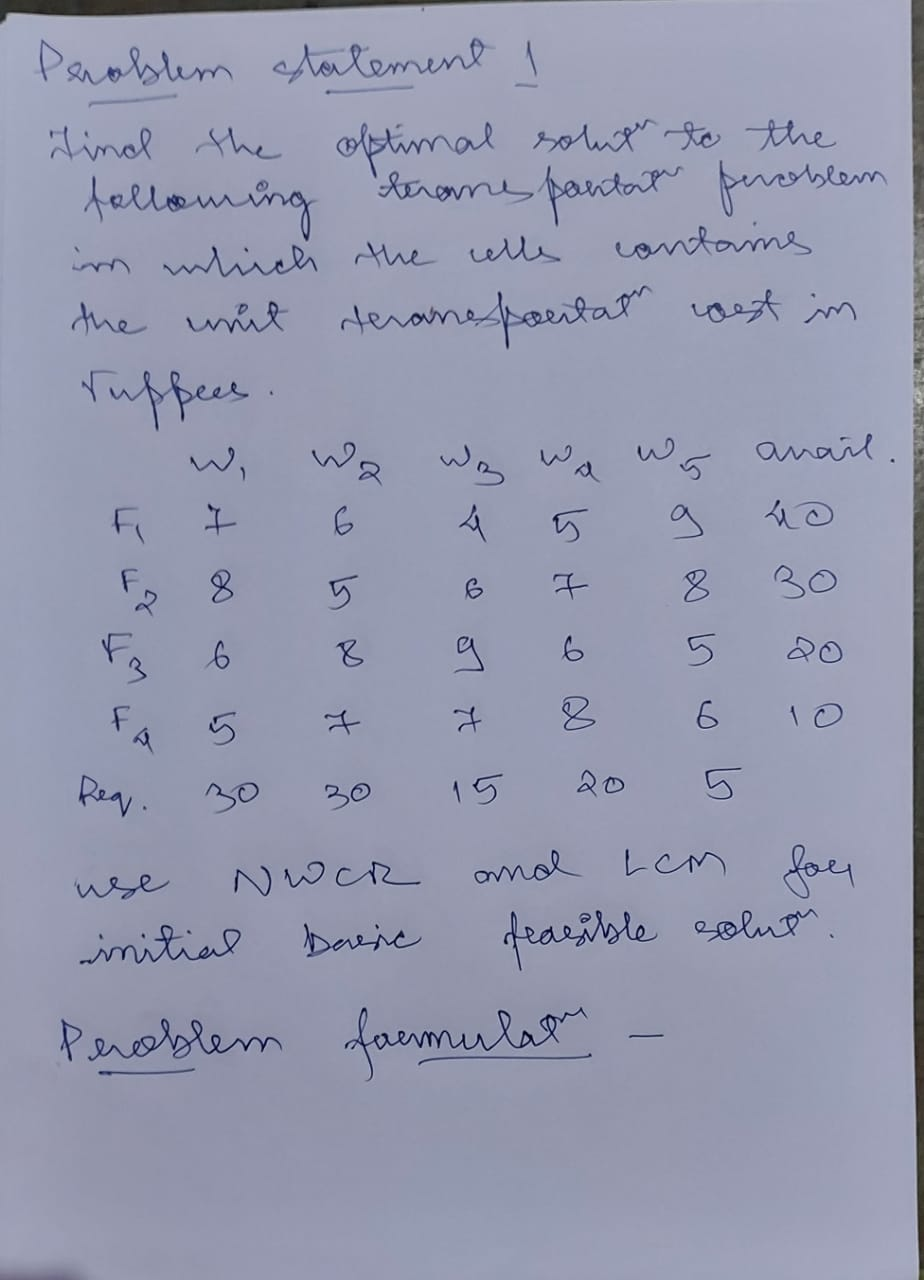
\includegraphics[width=\paperwidth, height=10in]{Page1}
\end{flushleft}
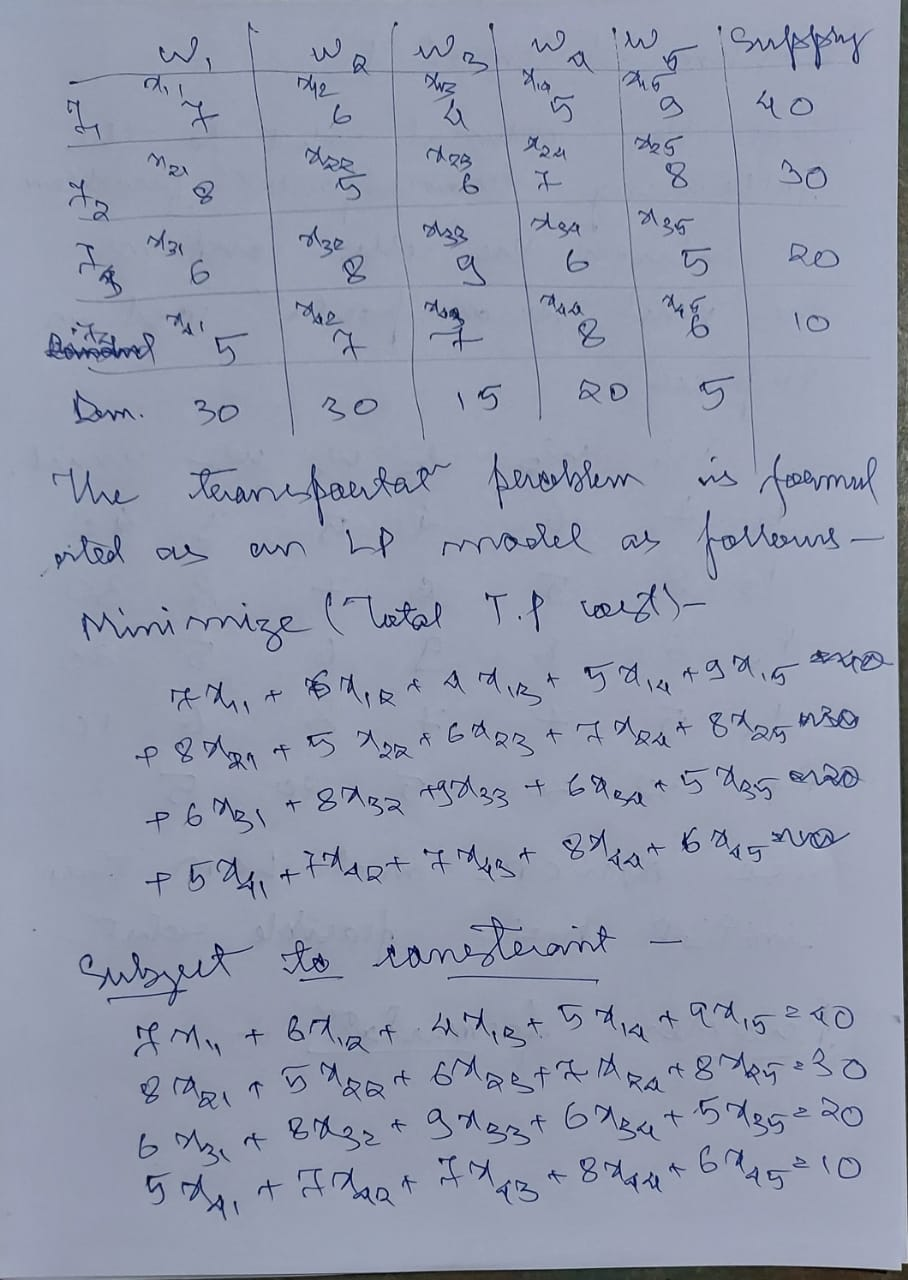
\includegraphics[width=\paperwidth, height=\paperheight]{Page2}
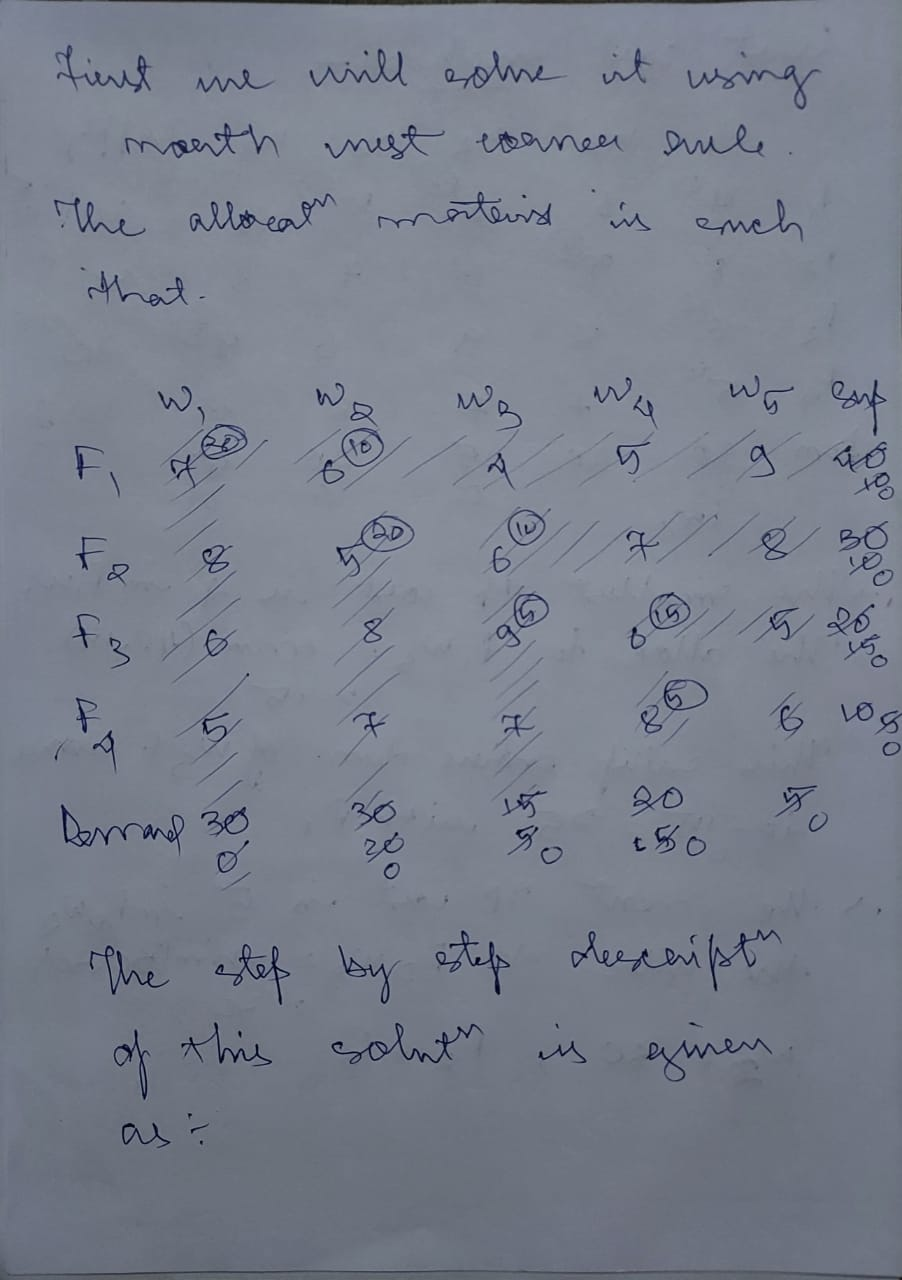
\includegraphics[width=\paperwidth, height=\paperheight]{Page3}
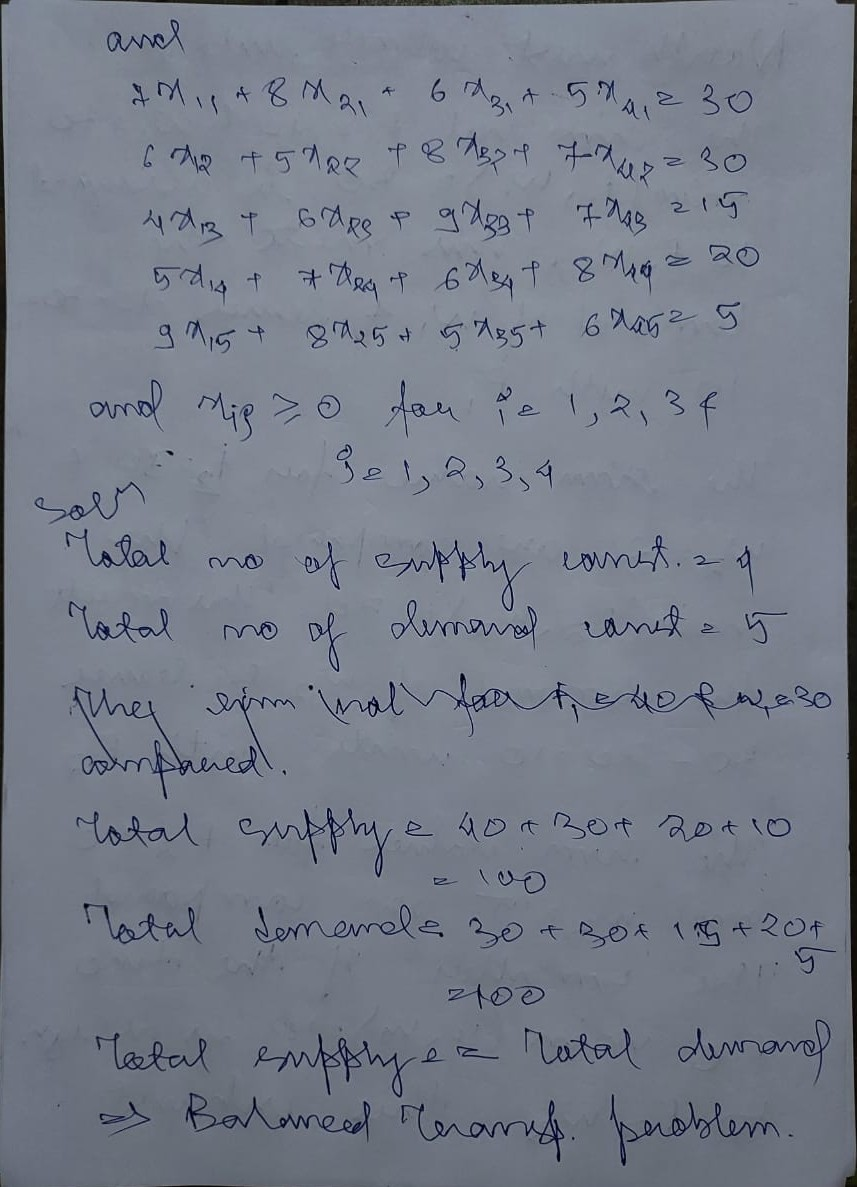
\includegraphics[width=\paperwidth, height=\paperheight]{Page4}
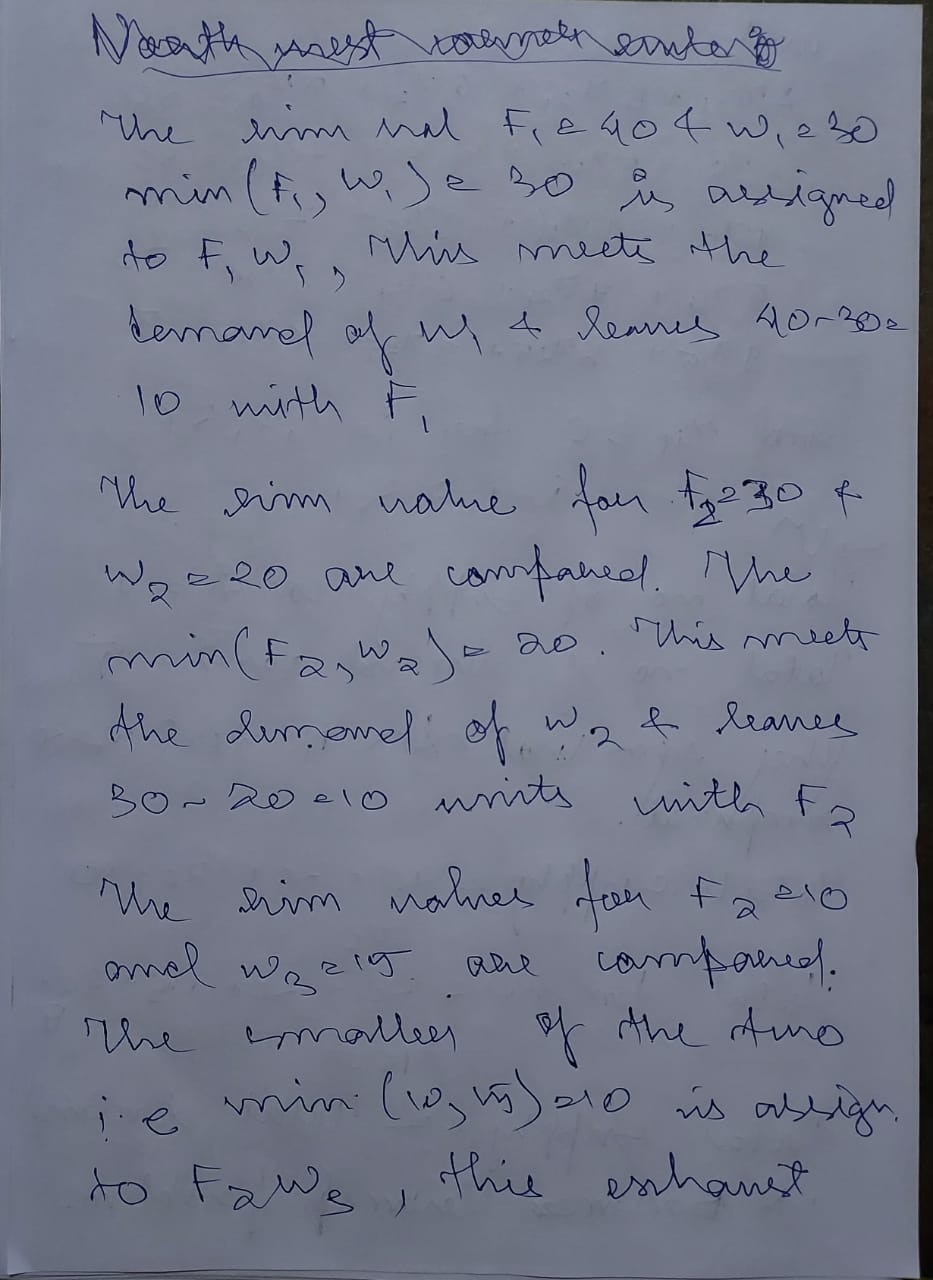
\includegraphics[width=\paperwidth, height=\paperheight]{Page5}
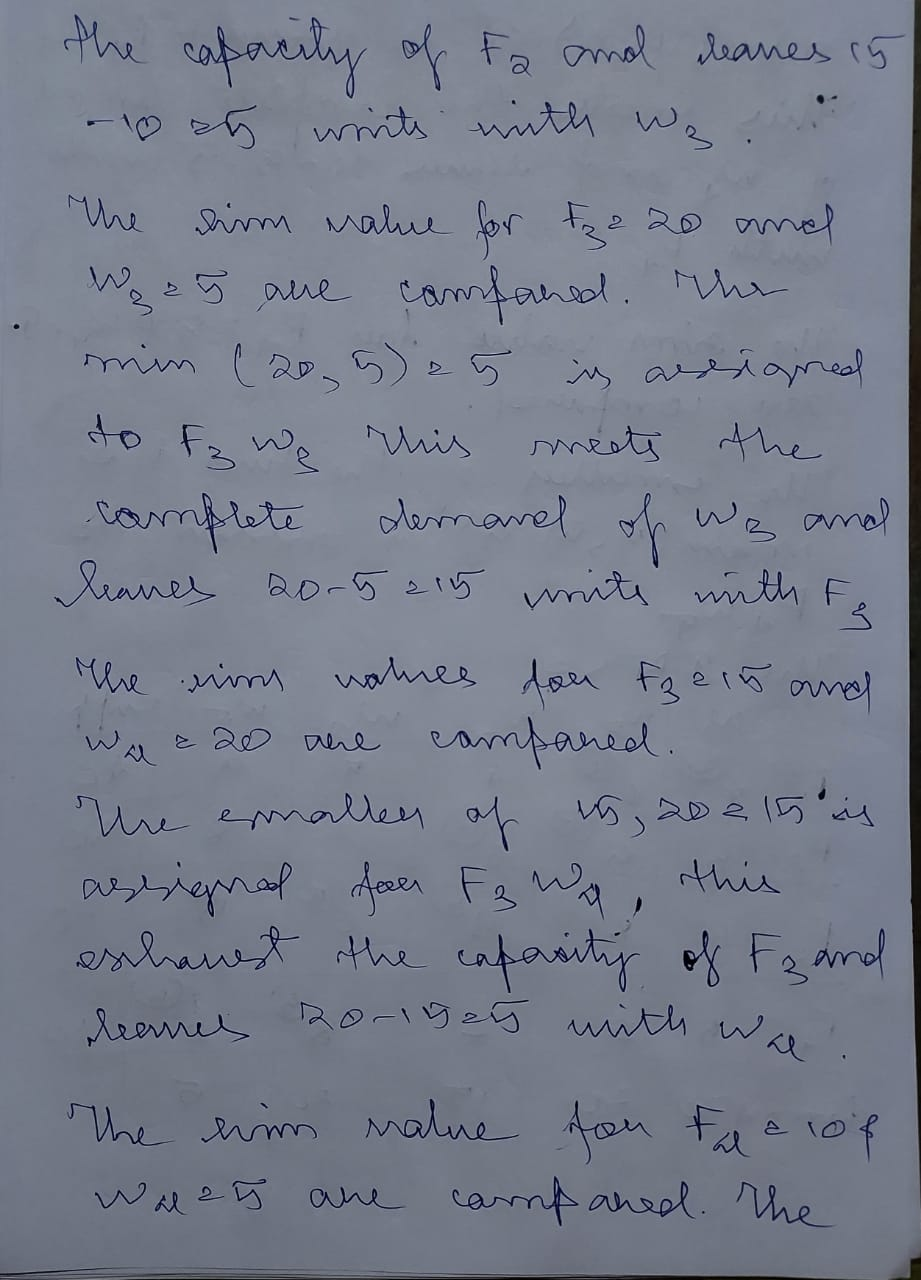
\includegraphics[width=\paperwidth, height=\paperheight]{Page6}
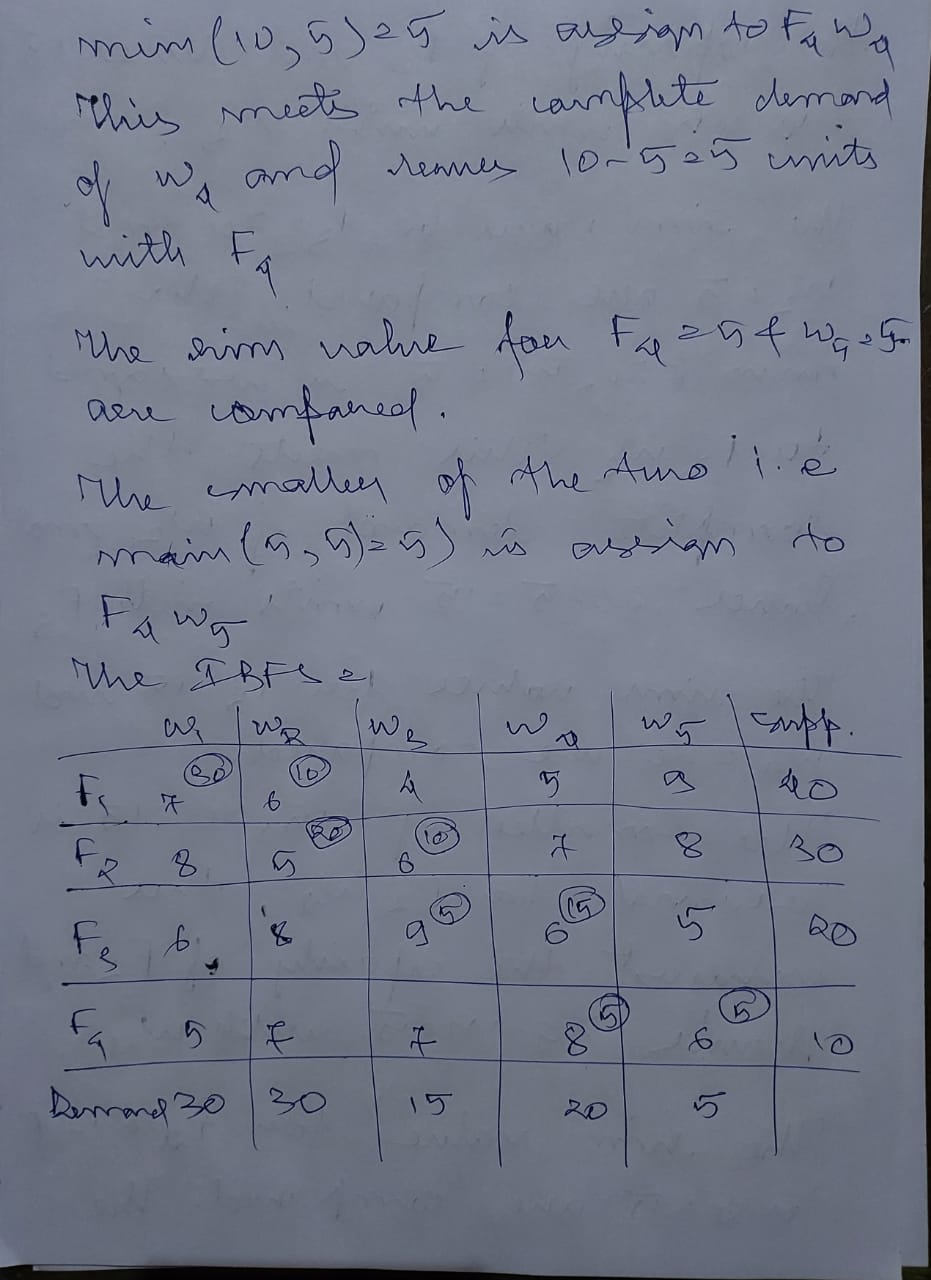
\includegraphics[width=\paperwidth, height=\paperheight]{Page7}
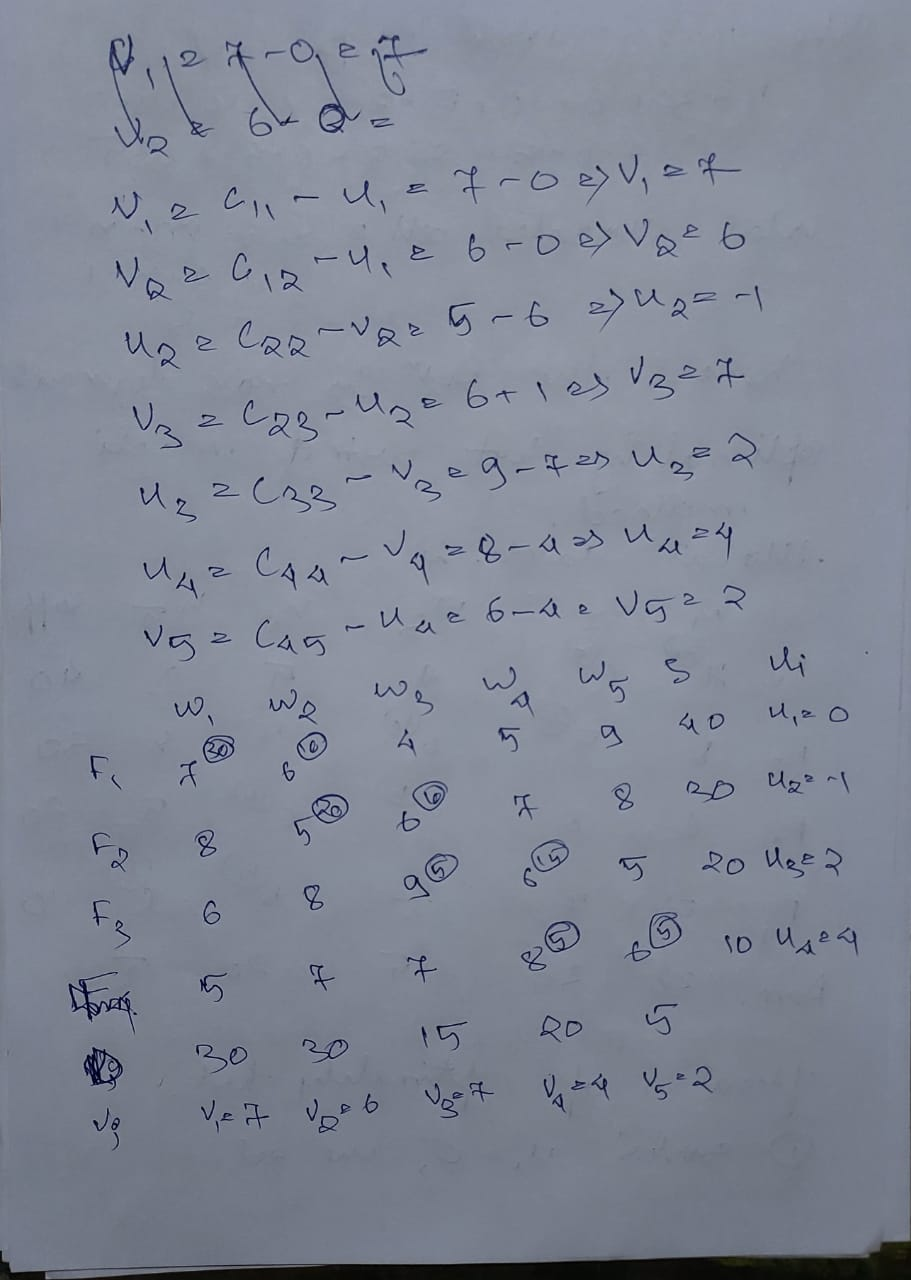
\includegraphics[width=\paperwidth, height=\paperheight]{Page8}
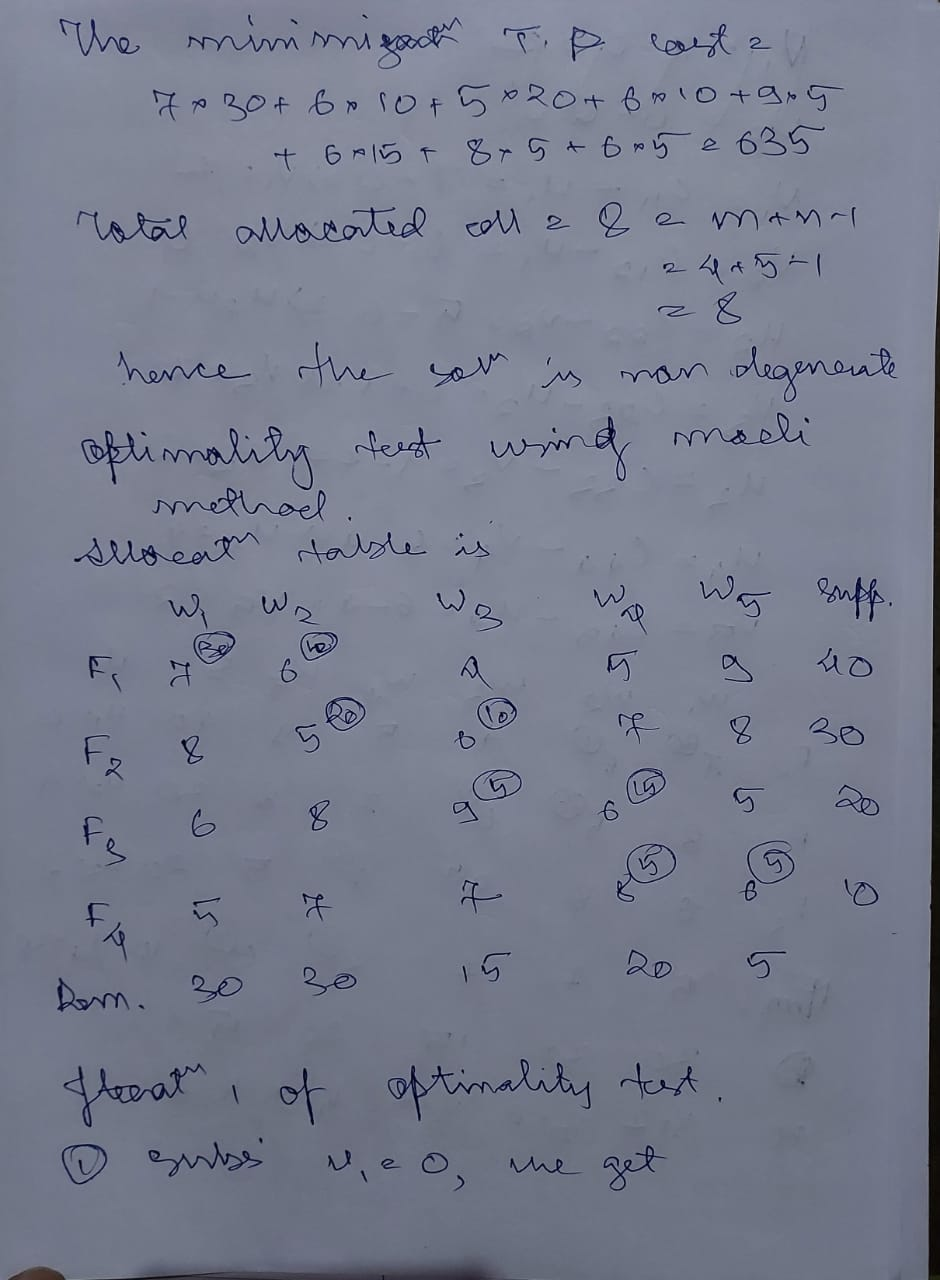
\includegraphics[width=\paperwidth, height=\paperheight]{Page9}
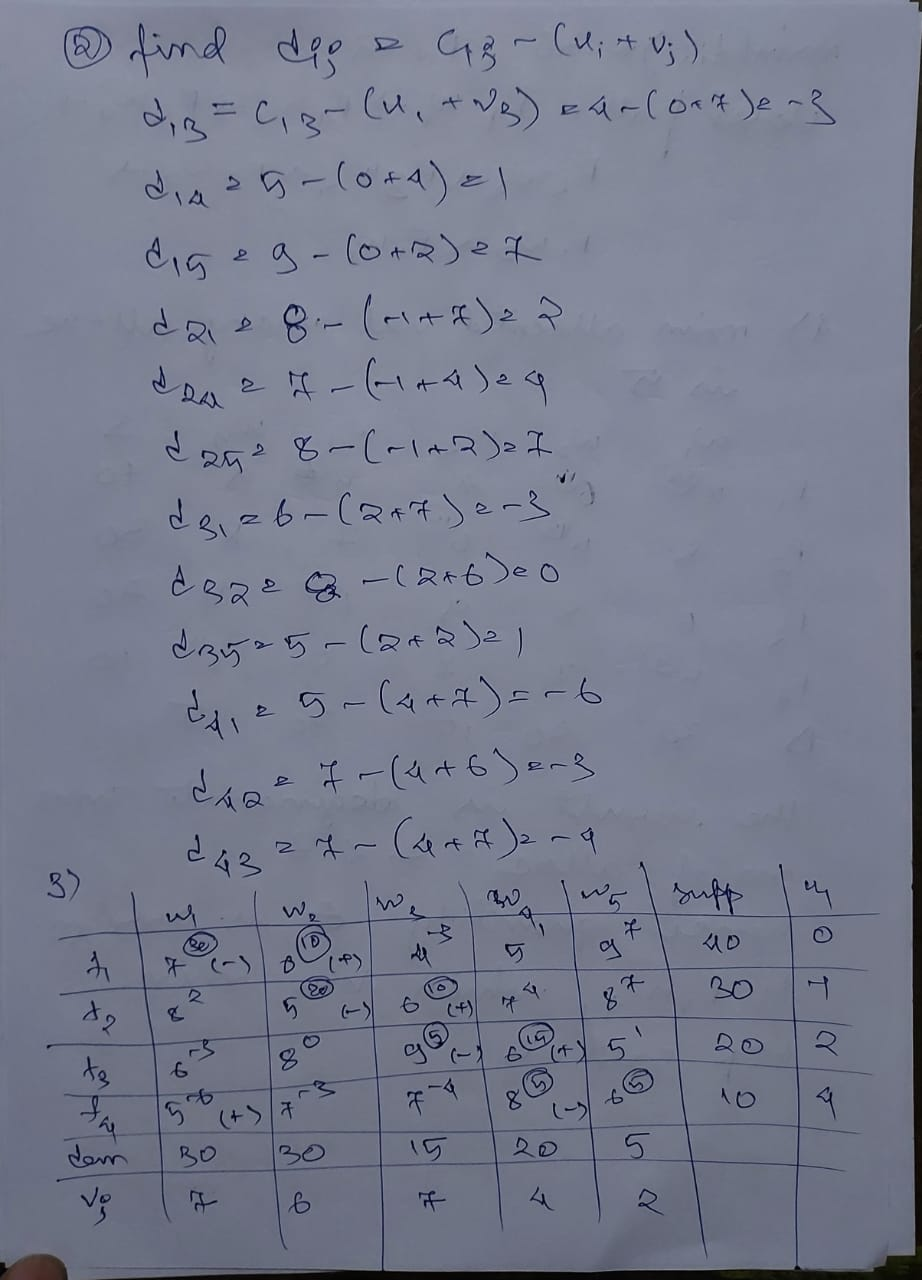
\includegraphics[width=\paperwidth, height=\paperheight]{Page10}
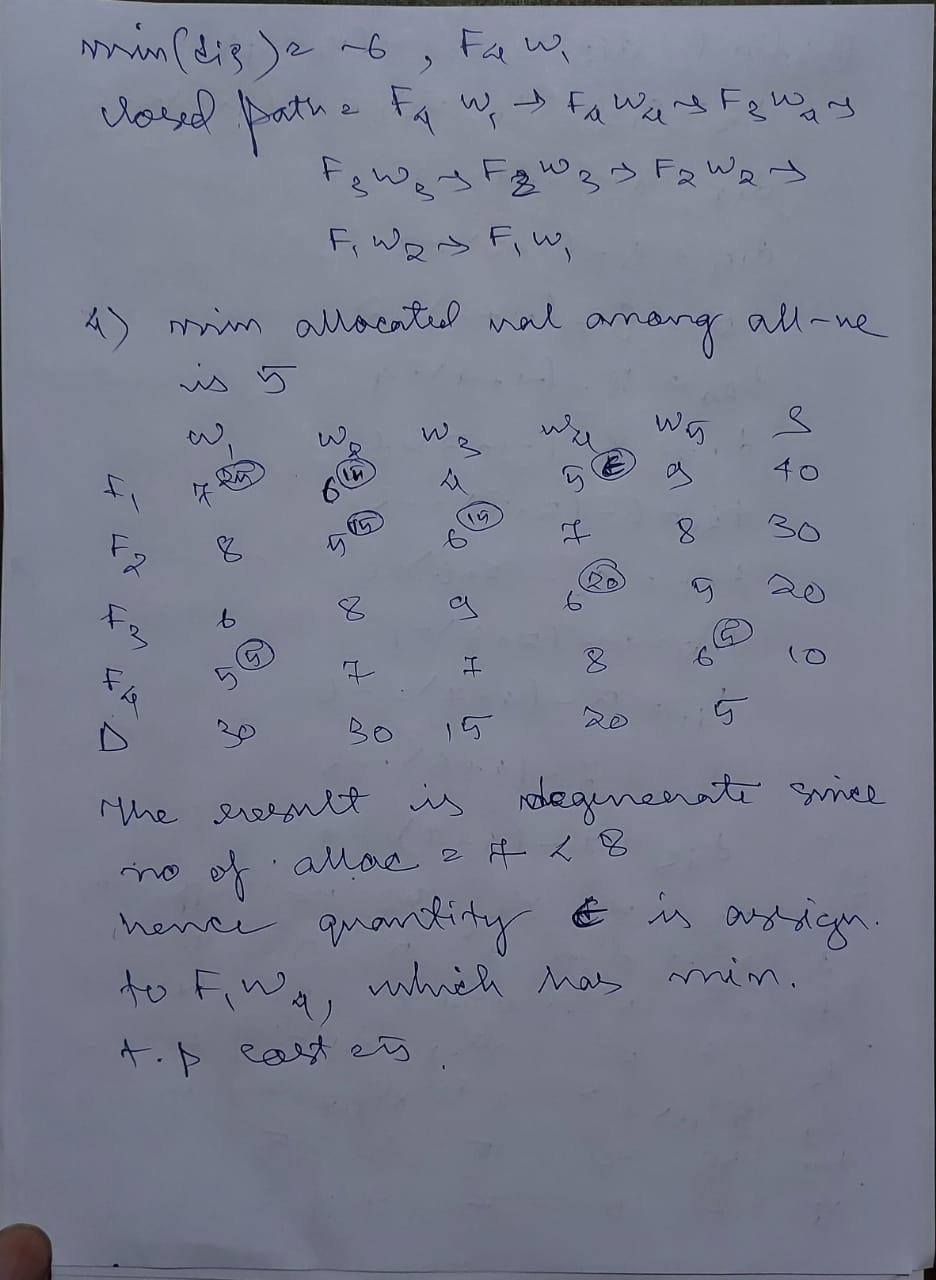
\includegraphics[width=\paperwidth, height=\paperheight]{Page11}
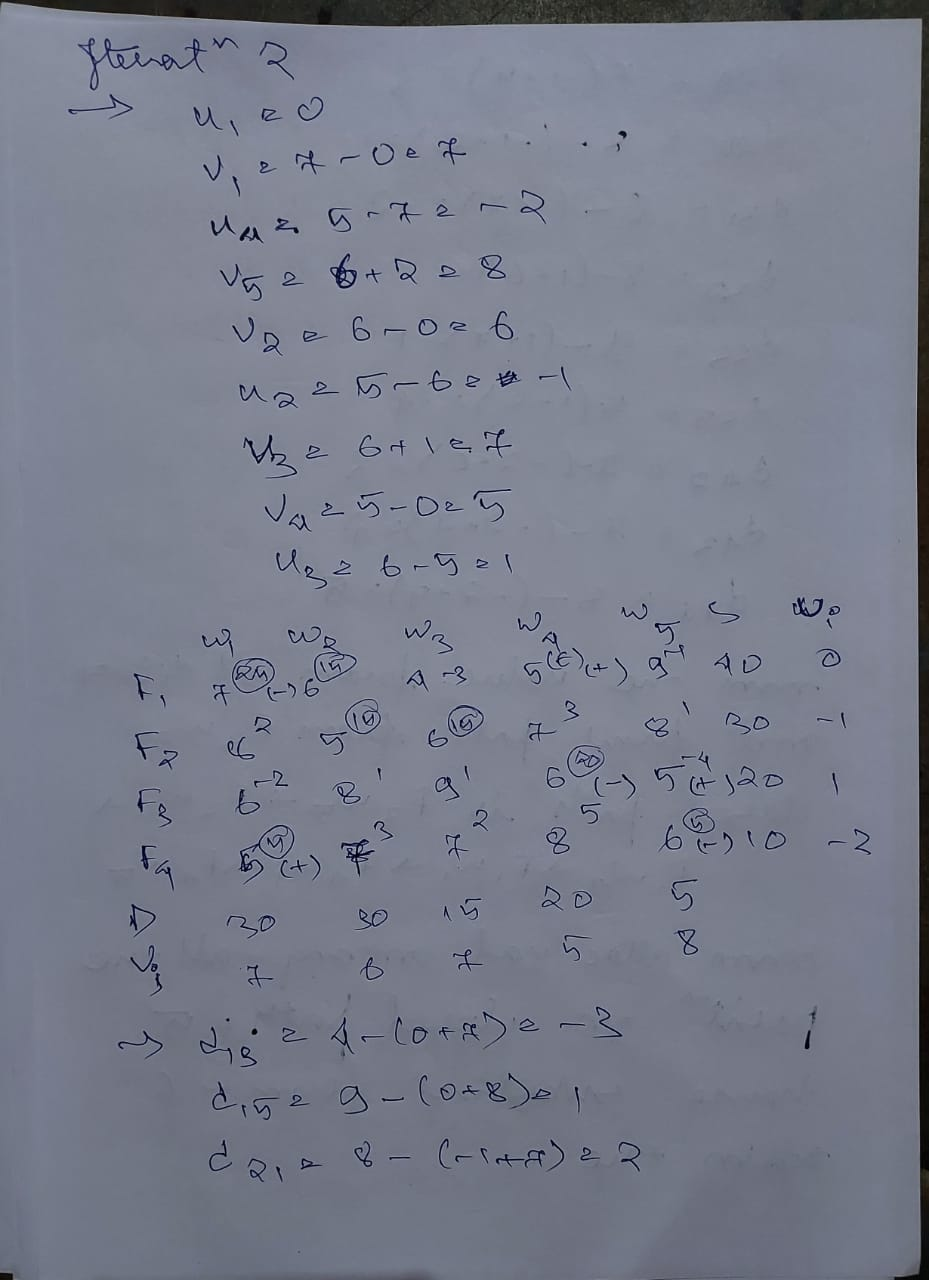
\includegraphics[width=\paperwidth, height=\paperheight]{Page12}
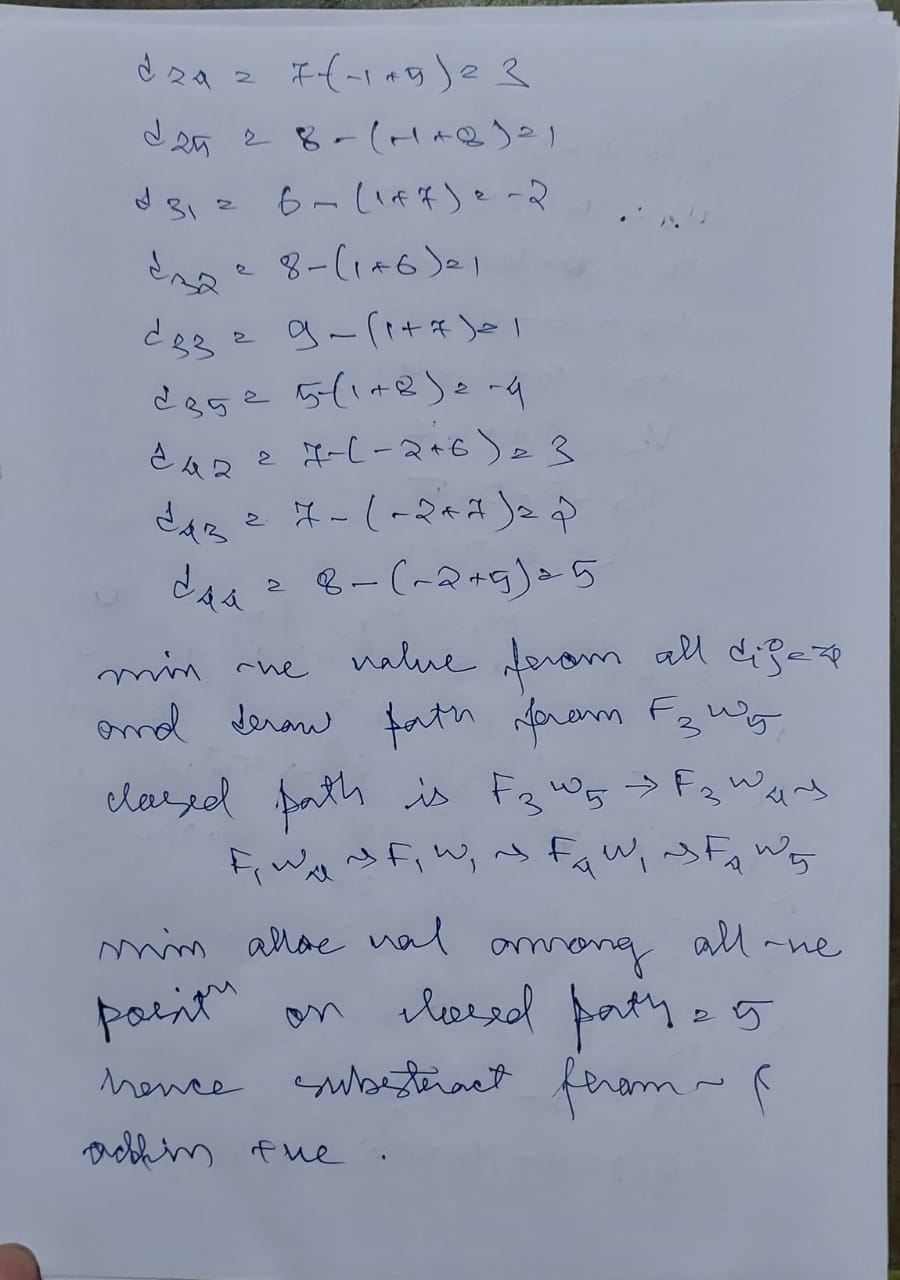
\includegraphics[width=\paperwidth, height=\paperheight]{Page13}
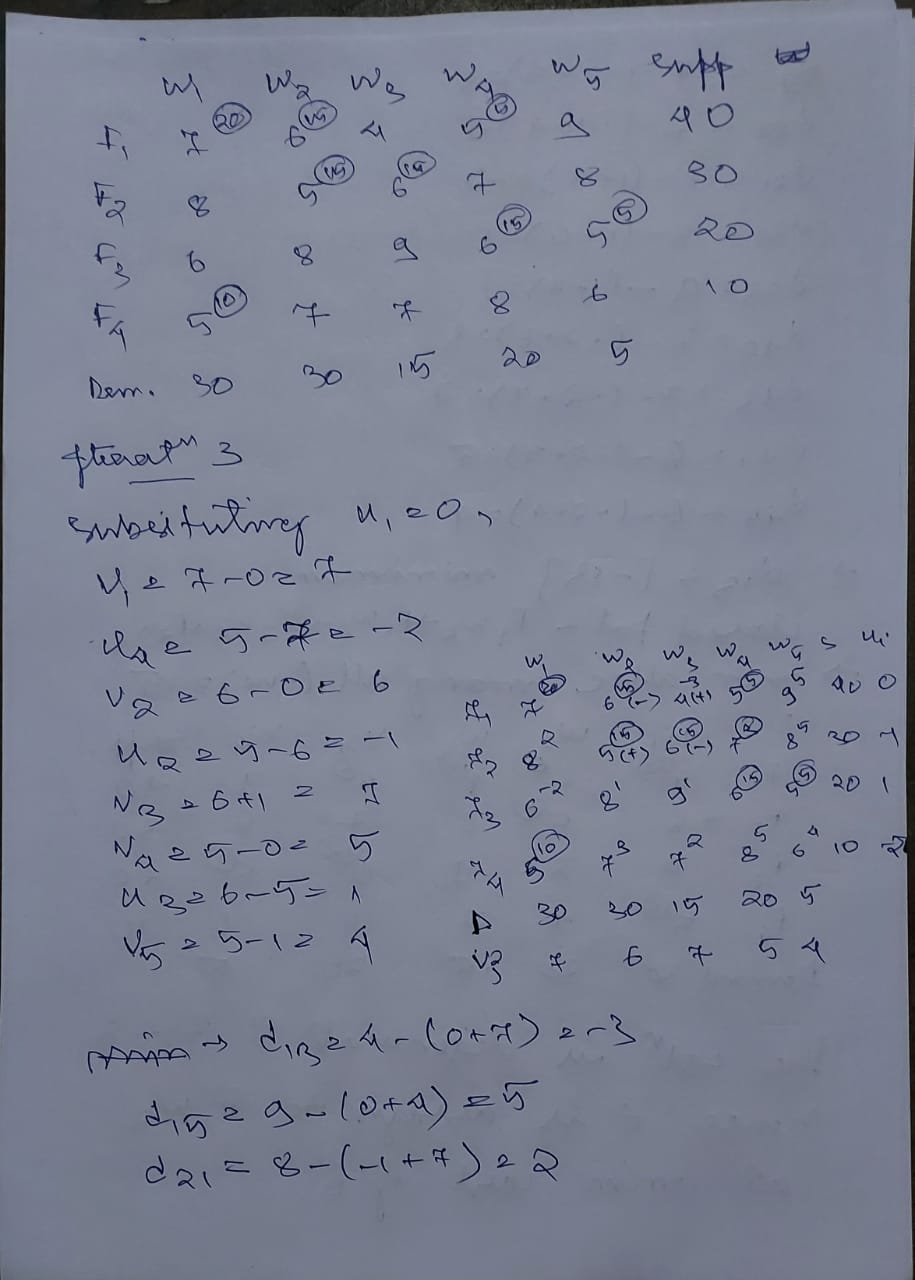
\includegraphics[width=\paperwidth, height=\paperheight]{Page14}
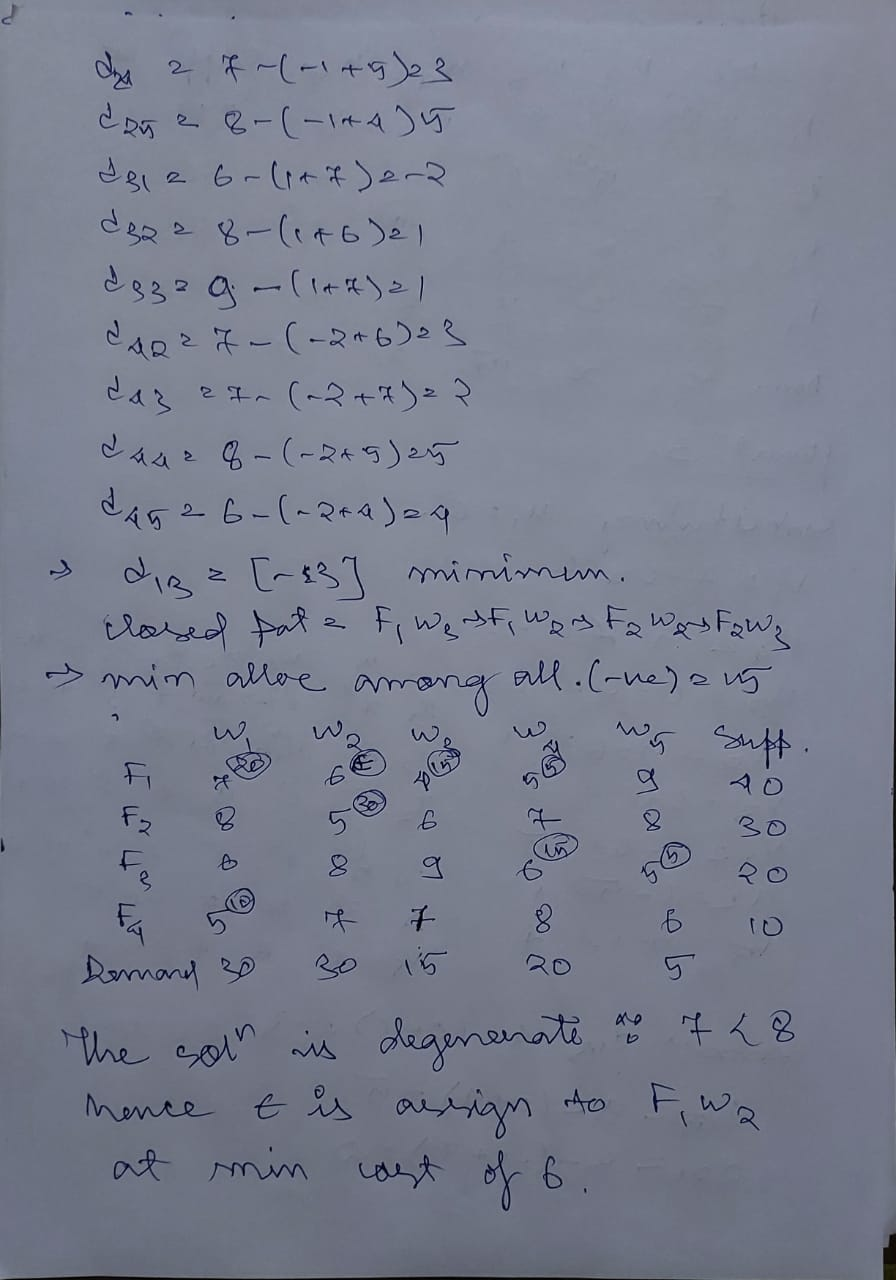
\includegraphics[width=\paperwidth, height=\paperheight]{Page15}
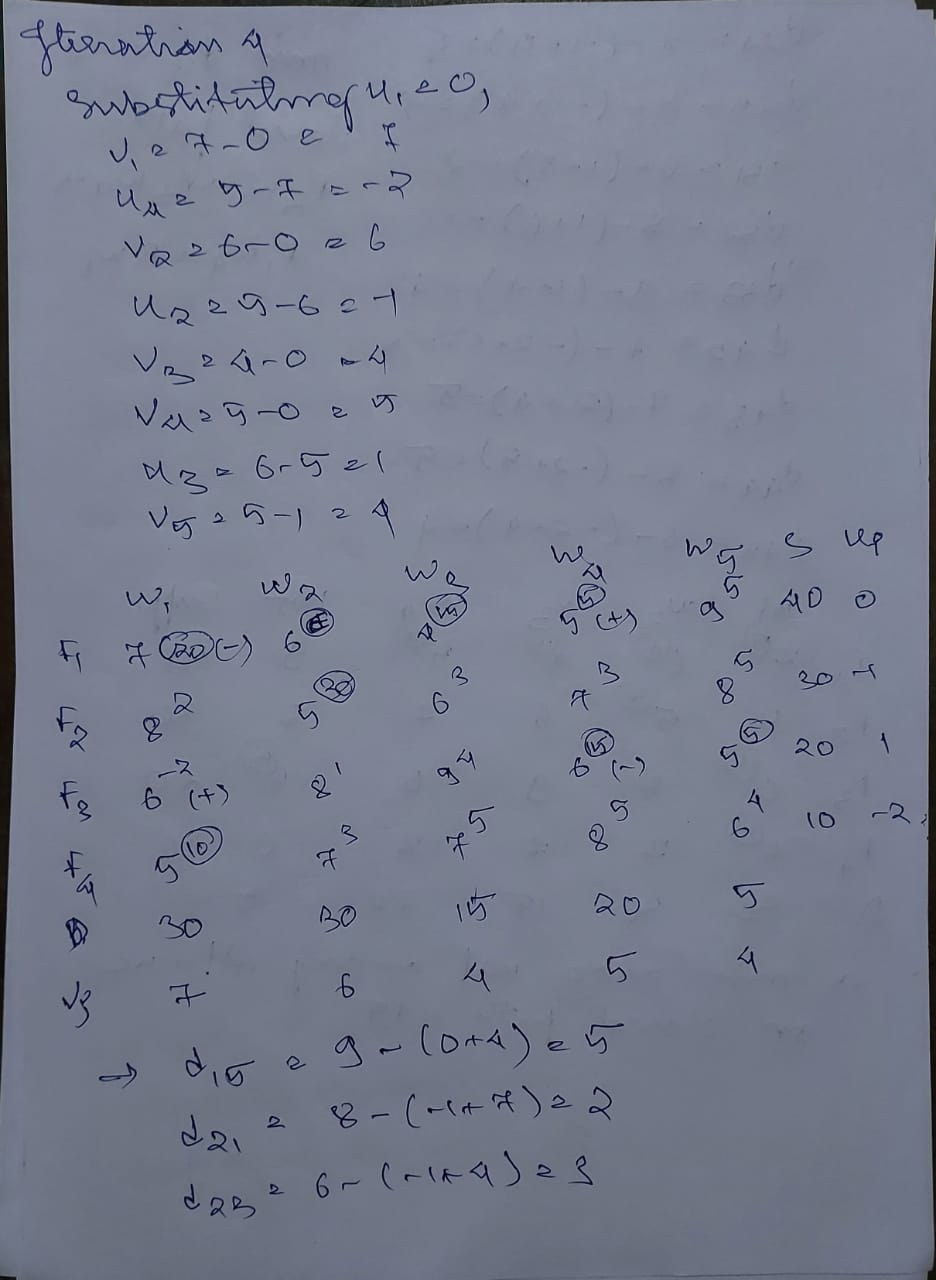
\includegraphics[width=\paperwidth, height=\paperheight]{Page16}
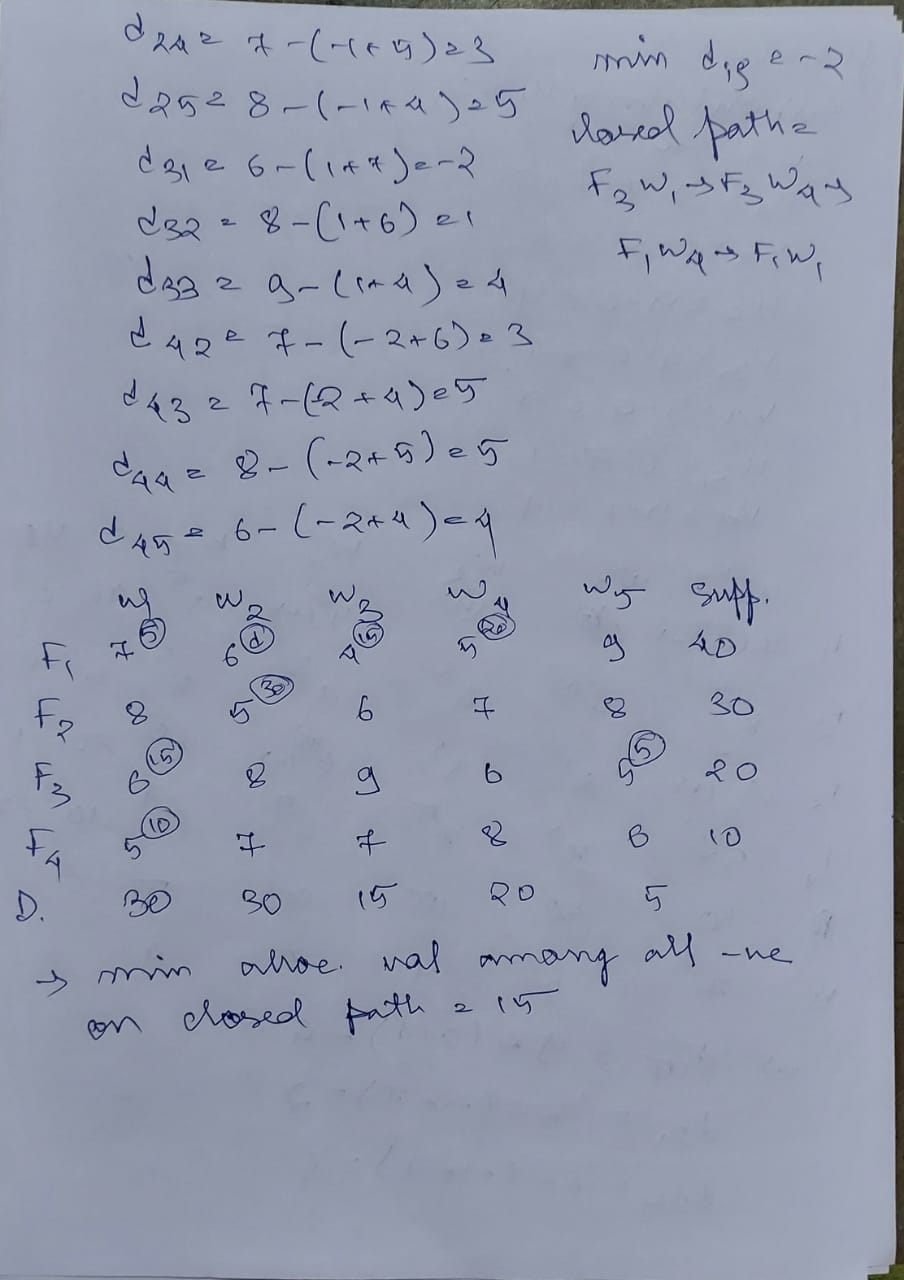
\includegraphics[width=\paperwidth, height=\paperheight]{Page17}
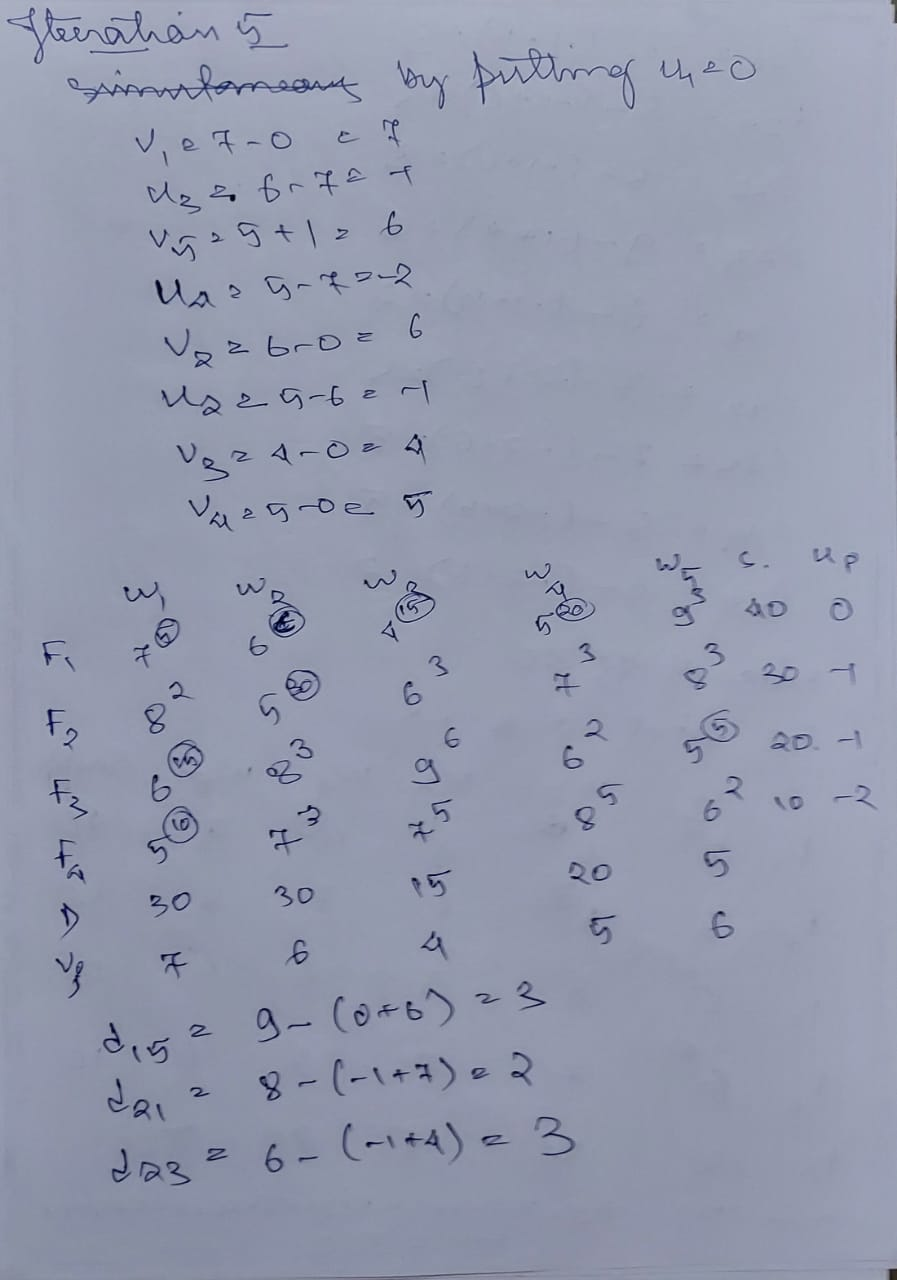
\includegraphics[width=\paperwidth, height=\paperheight]{Page18}
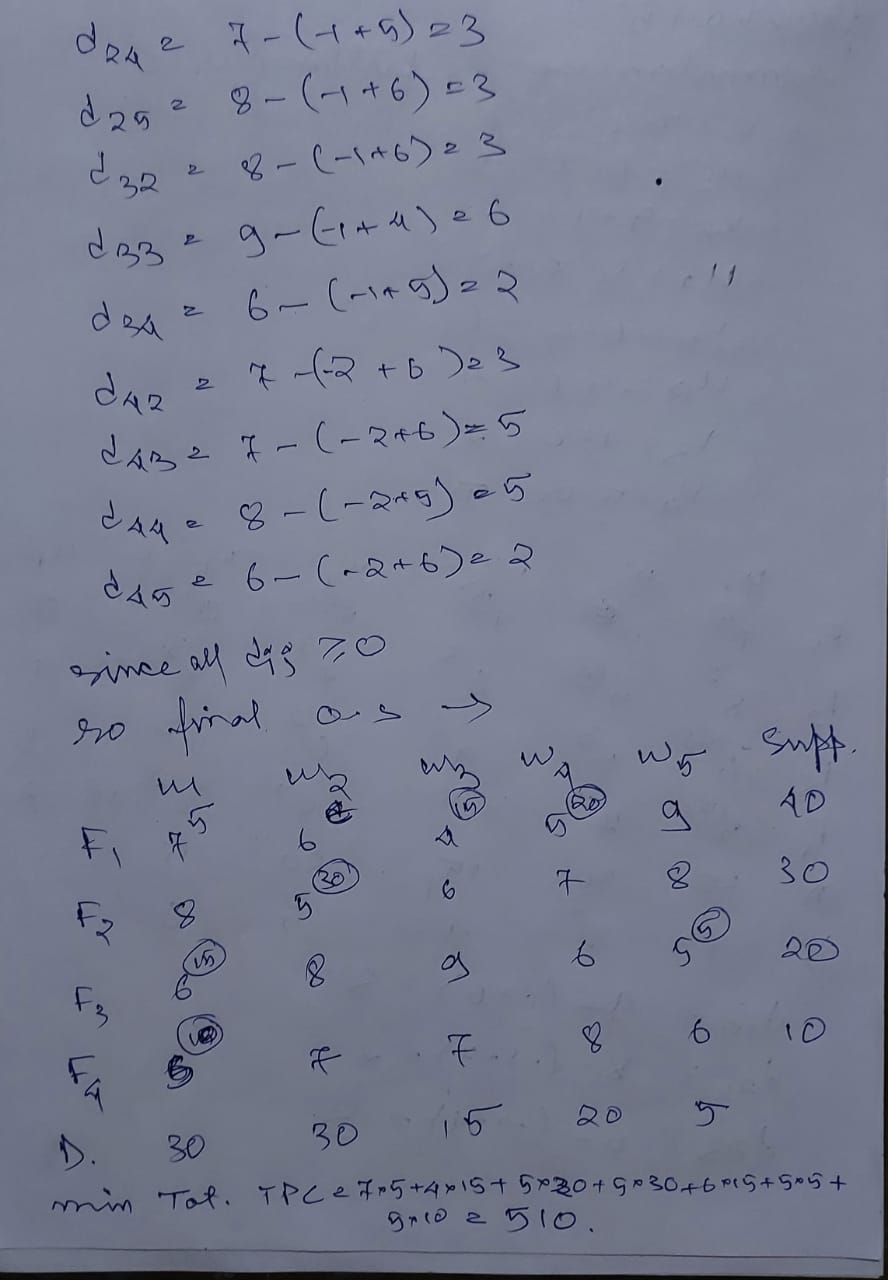
\includegraphics[width=\paperwidth, height=\paperheight]{Page19}
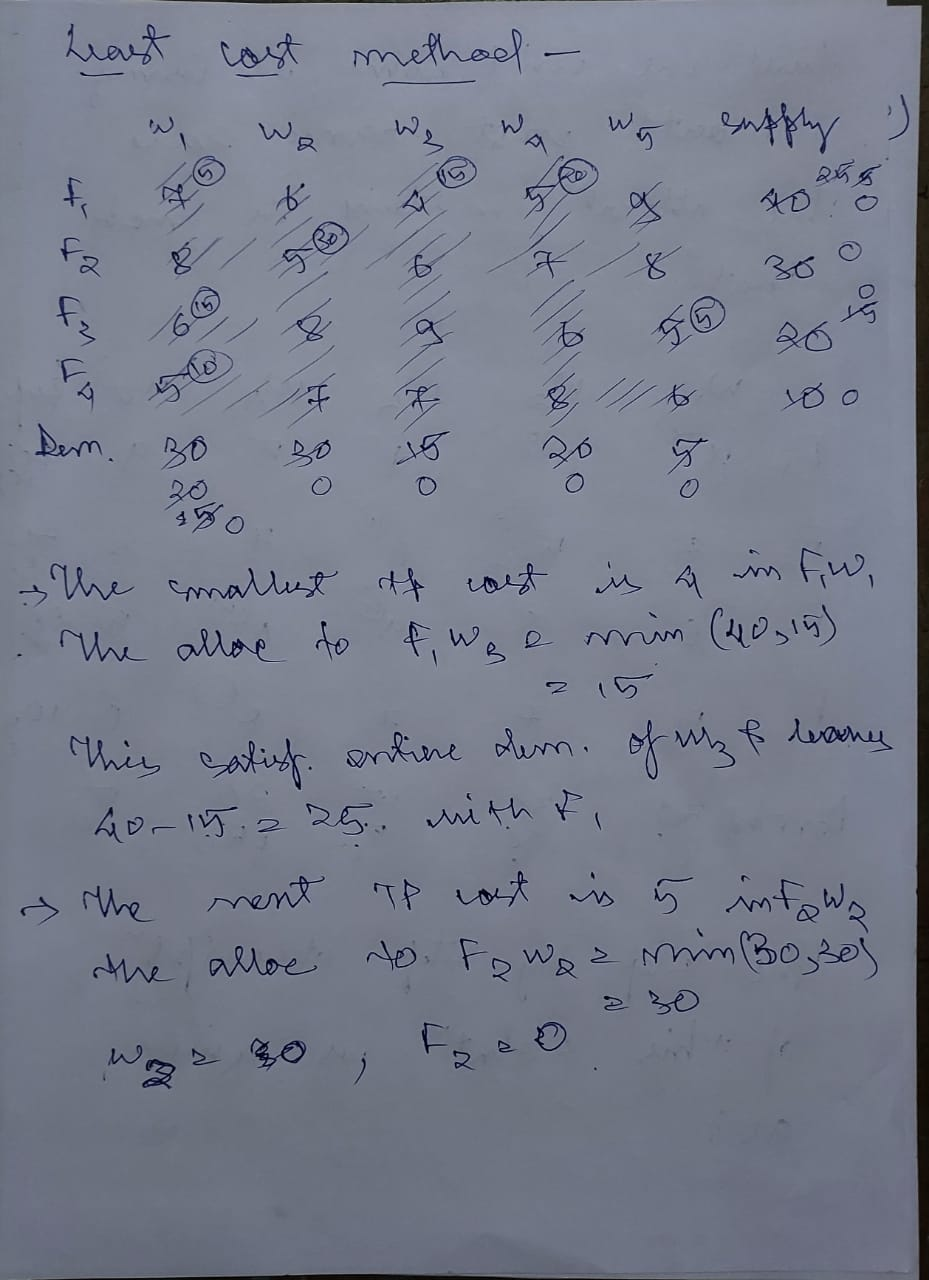
\includegraphics[width=\paperwidth, height=\paperheight]{Page20}
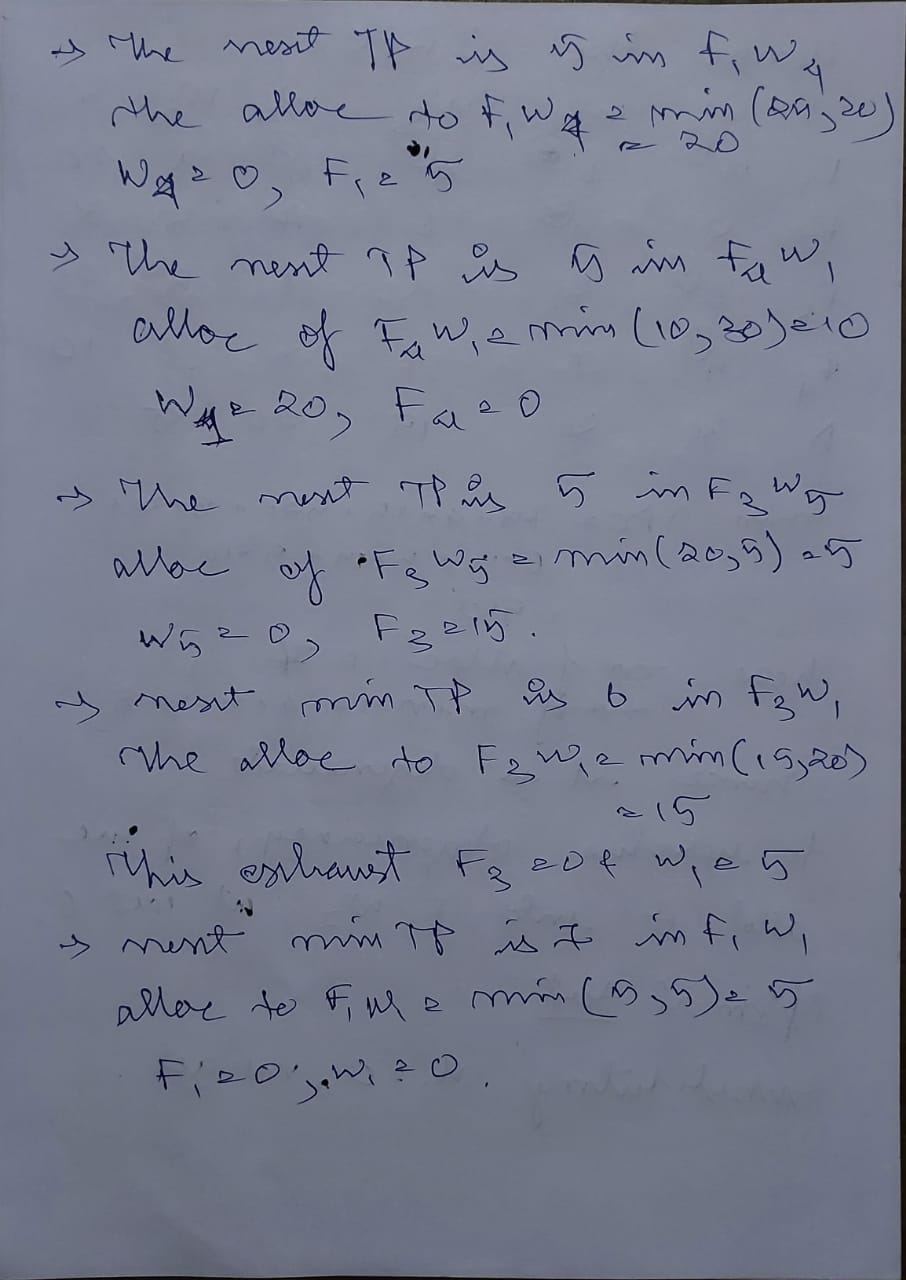
\includegraphics[width=\paperwidth, height=\paperheight]{Page21}
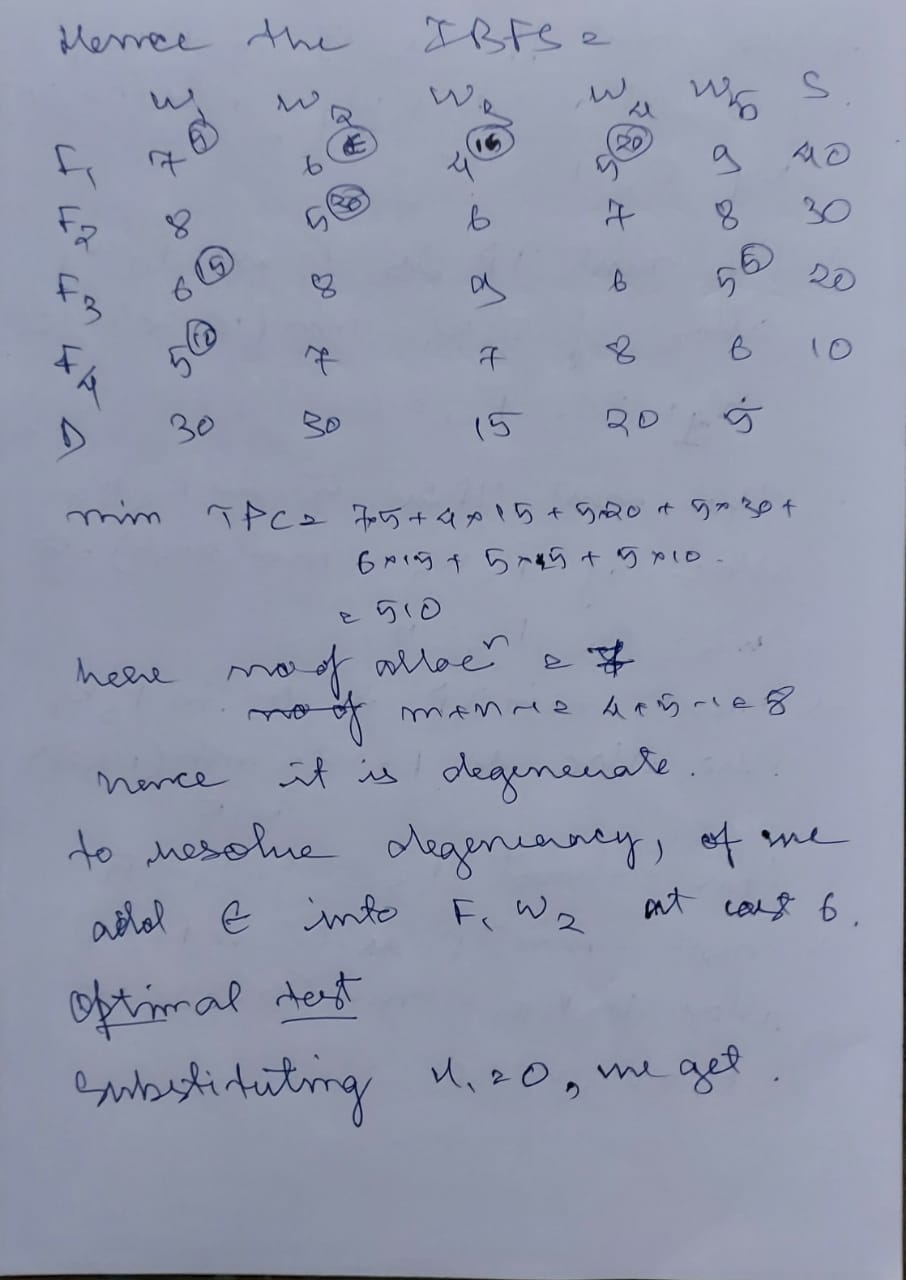
\includegraphics[width=\paperwidth, height=\paperheight]{Page22}
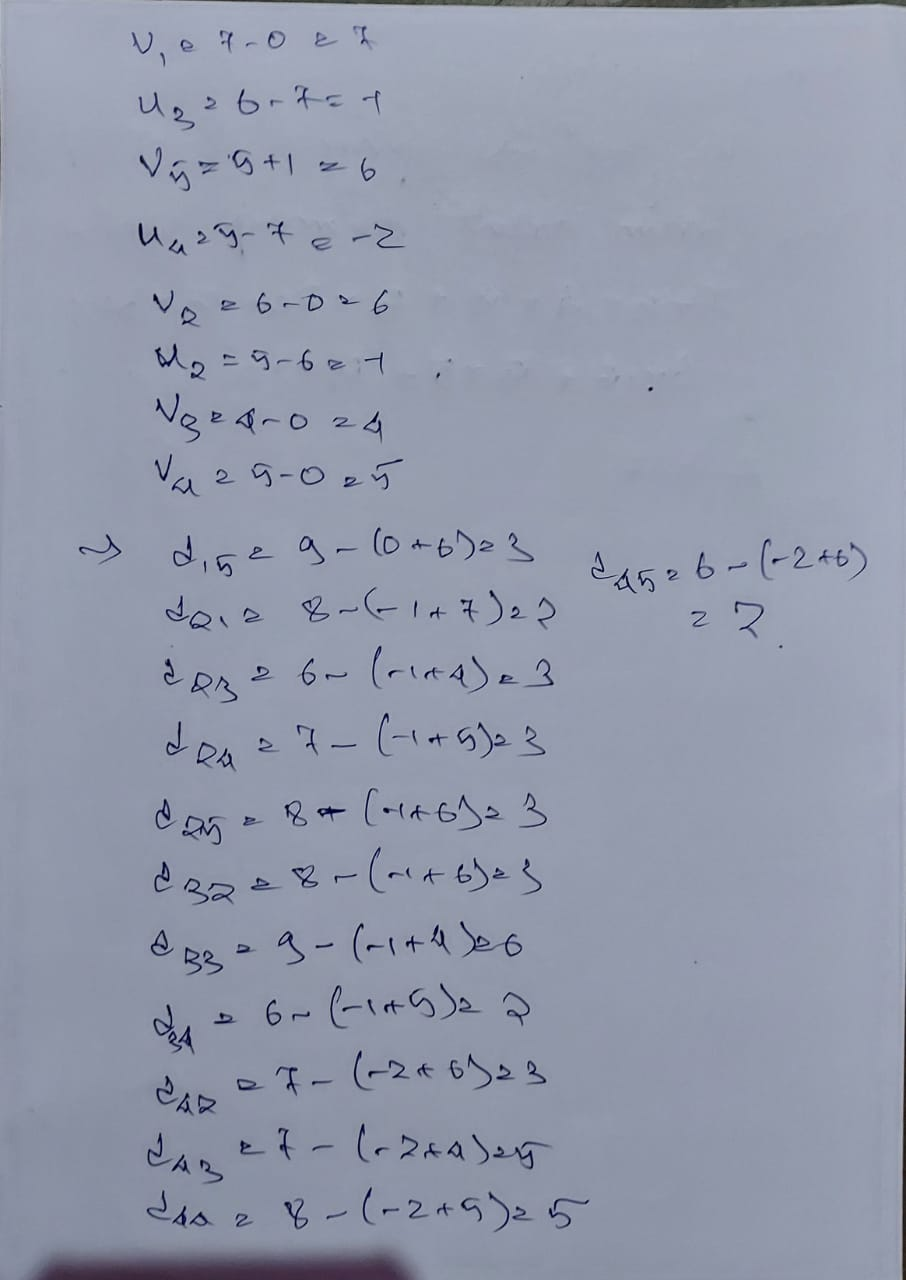
\includegraphics[width=\paperwidth, height=\paperheight]{Page23}
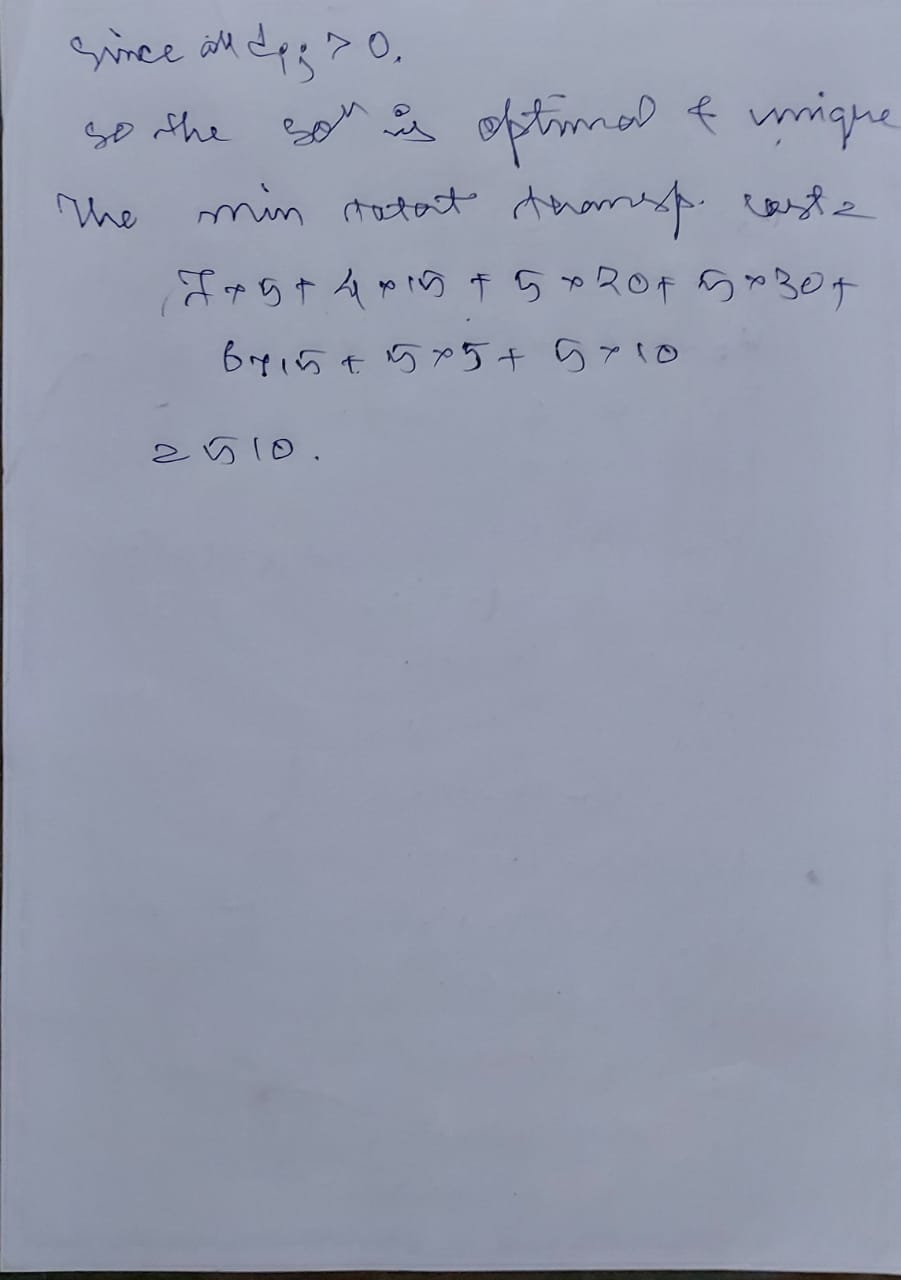
\includegraphics[width=\paperwidth, height=\paperheight]{Page24}
\begin{lstlisting}

	Python Code:

\end{lstlisting}
\lstinputlisting[language=Python]{PythonCode/assignment4problem1.py}
\pagebreak
\begin{lstlisting}

	Output:

\end{lstlisting}

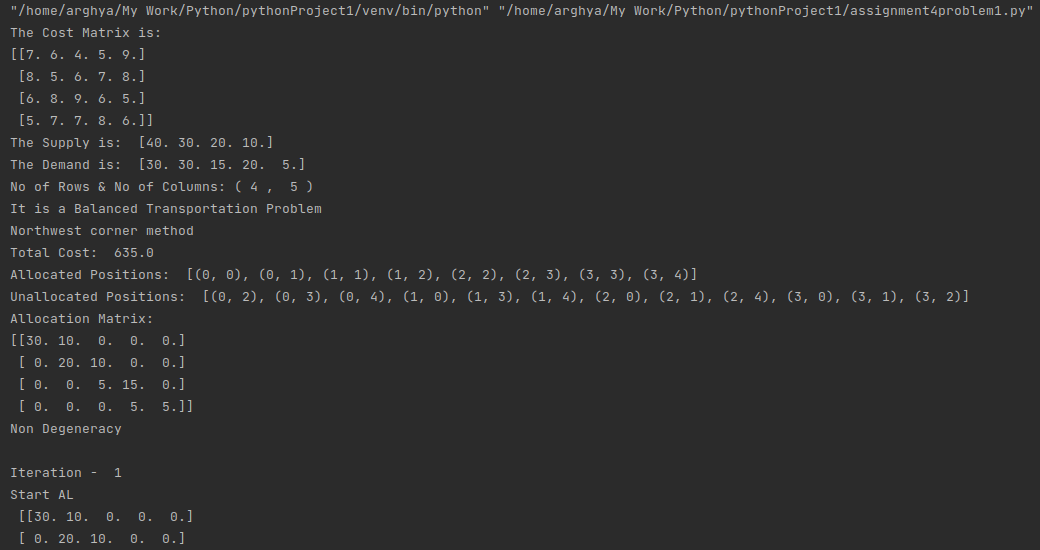
\includegraphics[width=550pt]{Output1}

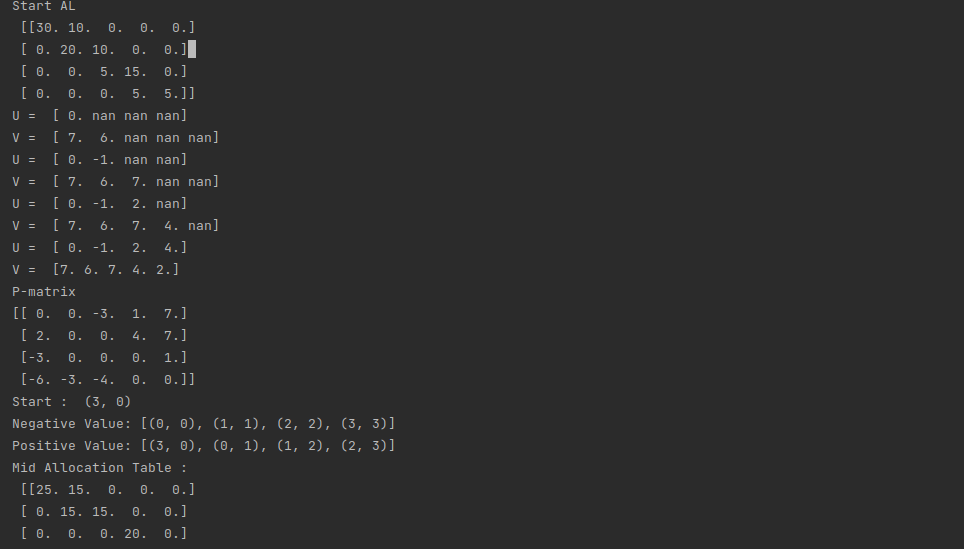
\includegraphics[width=550pt]{Output2}

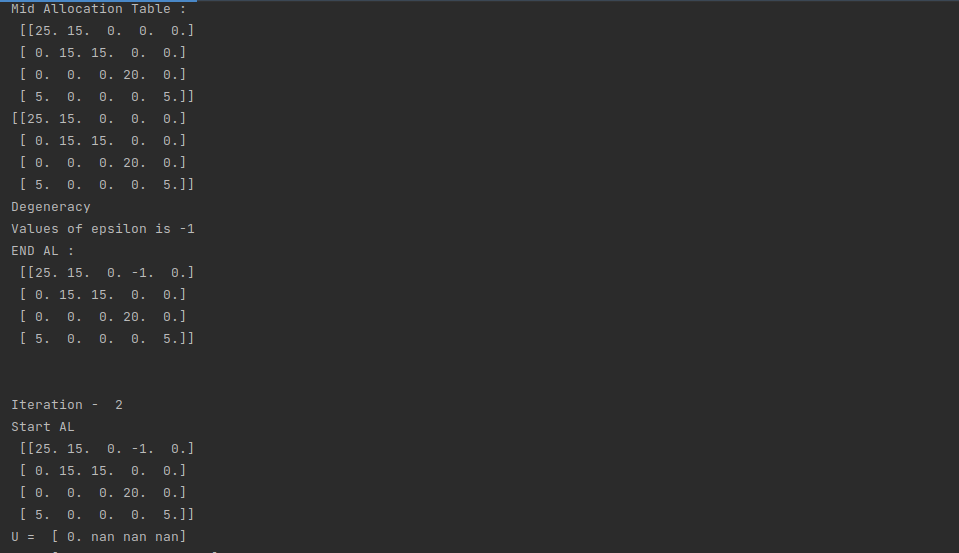
\includegraphics[width=550pt]{Output3}

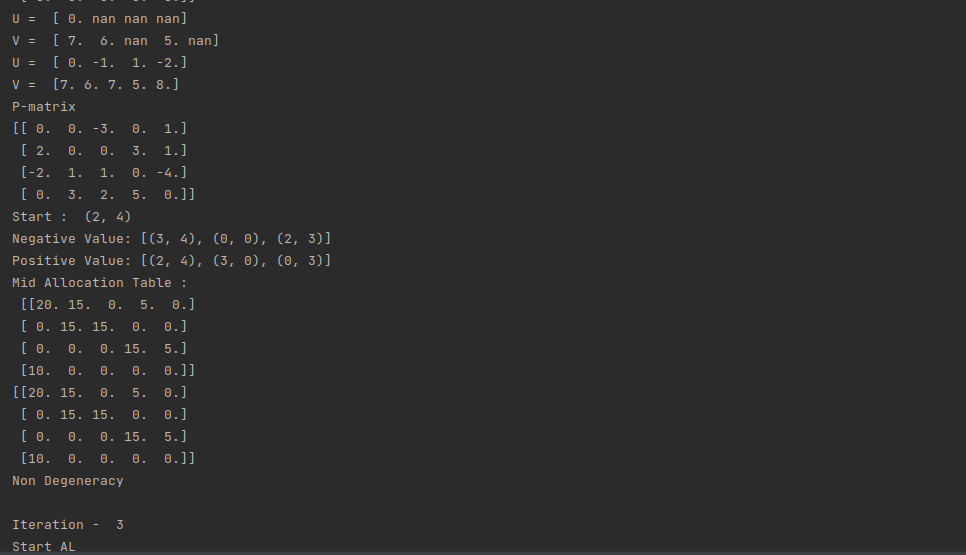
\includegraphics[width=550pt]{Output4}

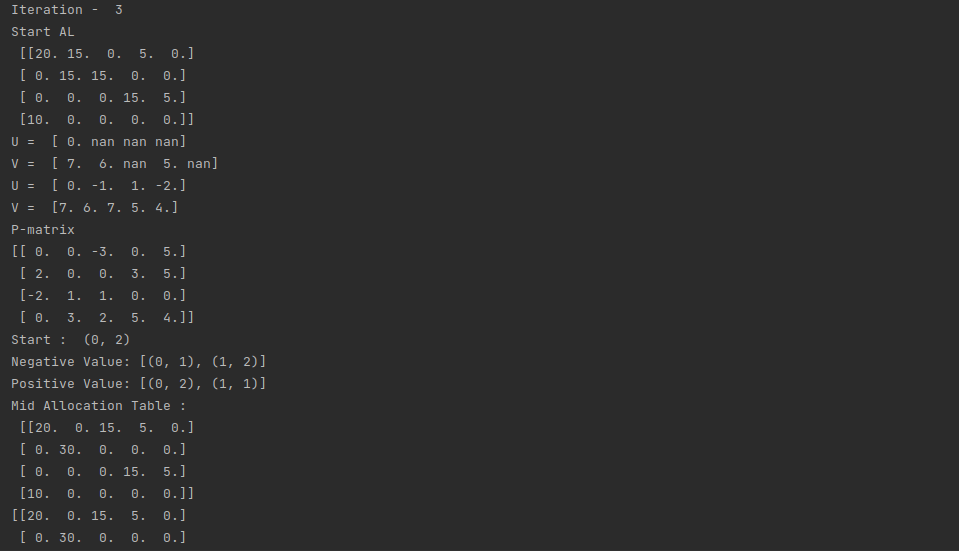
\includegraphics[width=550pt]{Output5}

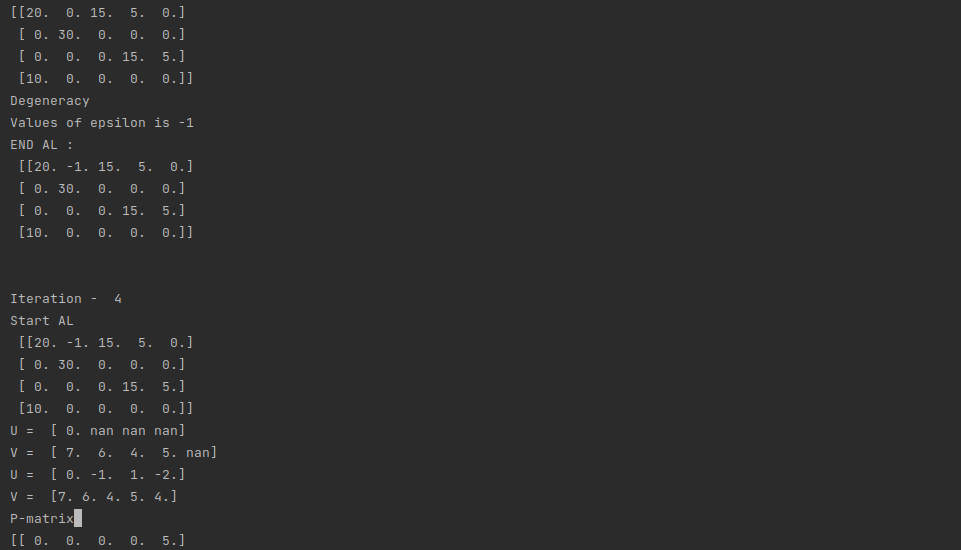
\includegraphics[width=550pt]{Output6}

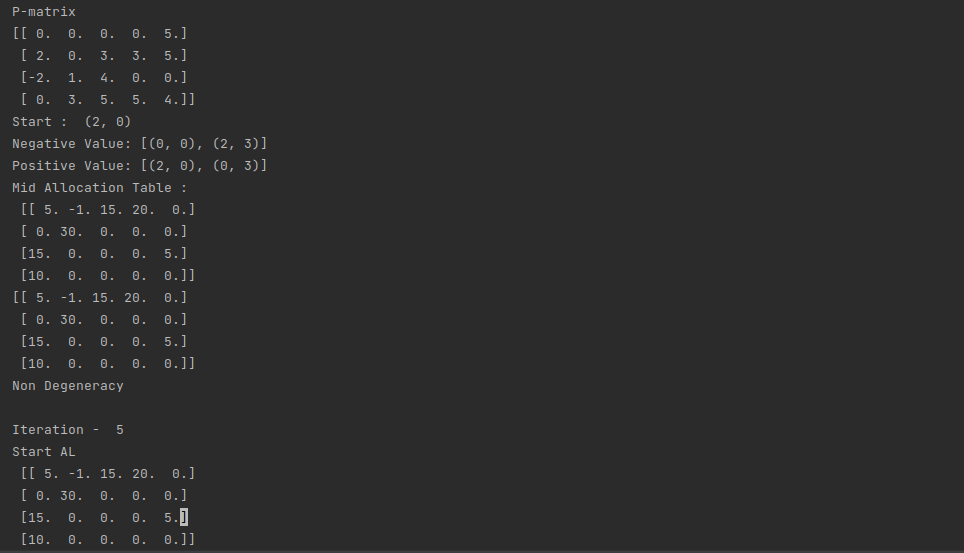
\includegraphics[width=550pt]{Output7}

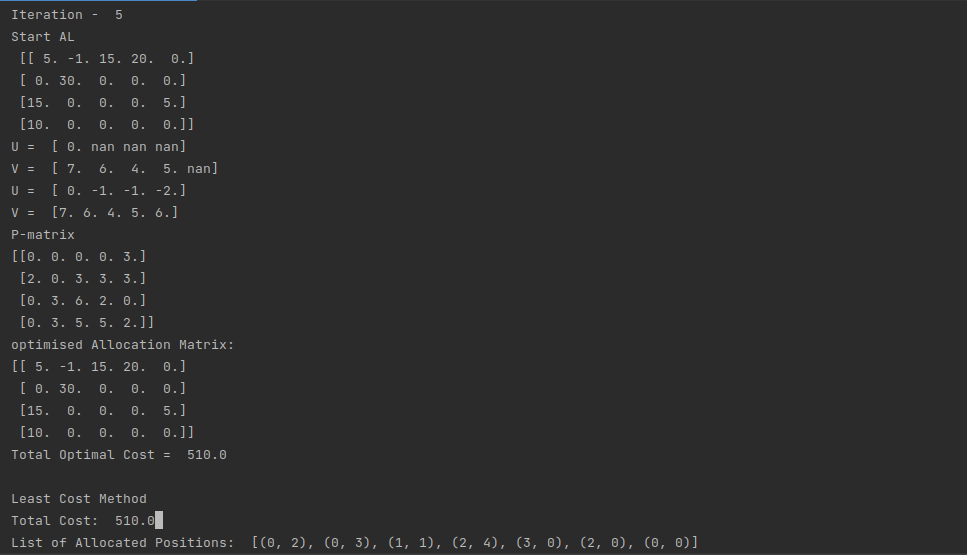
\includegraphics[width=550pt]{Output8}

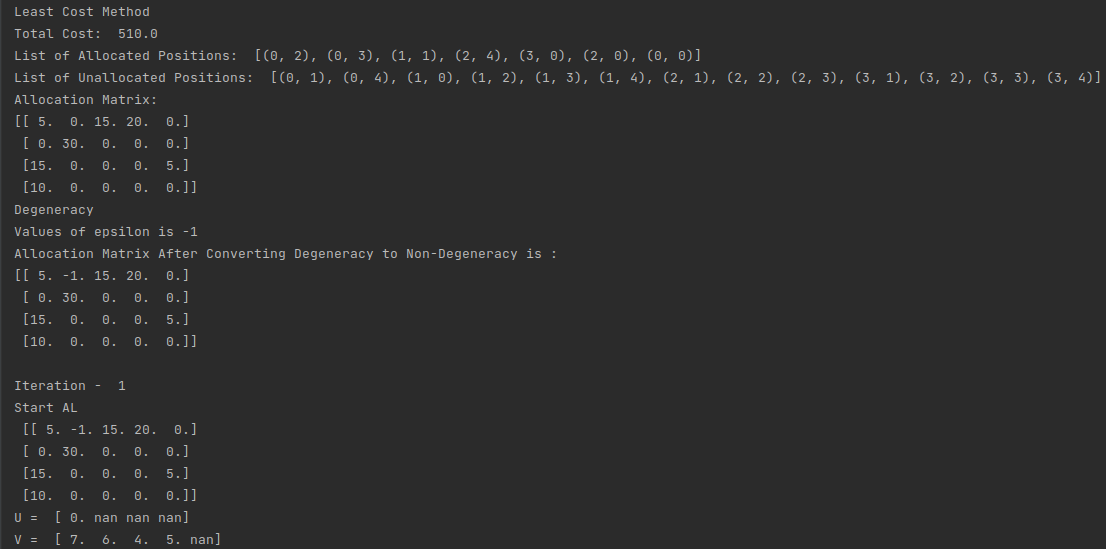
\includegraphics[width=550pt]{Output9}

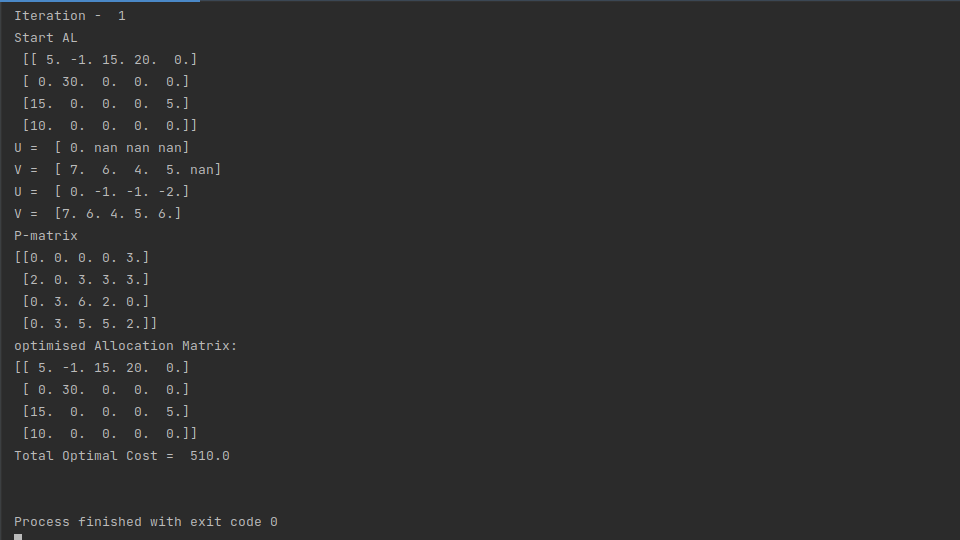
\includegraphics[width=550pt]{Output10}

\pagebreak
\end{document}
